\chapter{Experiments and Results}
%%%%%%%%%%%%%%%%%%%%%%%%%%%%%%%%%%%%%%%%%%%%%%%%%%%%%%%%%%%%
%%%%%%%%%%%%%%%%%%%%  NEW SECTION   %%%%%%%%%%%%%%%%%%%%%%%%
%%%%%%%%%%%%%%%%%%%%%%%%%%%%%%%%%%%%%%%%%%%%%%%%%%%%%%%%%%%%
\setcounter{equation}{0}
The authors collected data for evaluating the performance of the
improved computer vision based navigation method. The test
was done in December 2019 in Trondheim, Norway, with
snowy conditions. They started navigating outdoors, entered an
office building where they walked around for five minutes, and
ended the data collection outdoors. Figure 4.1 shows the test
conditions outdoors. The whole experiment lasted approximately 13 minutes and resulted in 6740 images, the whole
route, computed with the reference solution, is shown in
Figure 4.2. RealSense depth camera provides RGB and depth
images separately, and this system aligned them at the time
of capture. Image rate varied between 1Hz and 15Hz, 8Hz on
average, however this was accommodated using time stamps
from image processing.\\
\begin{figure}
    \centering
    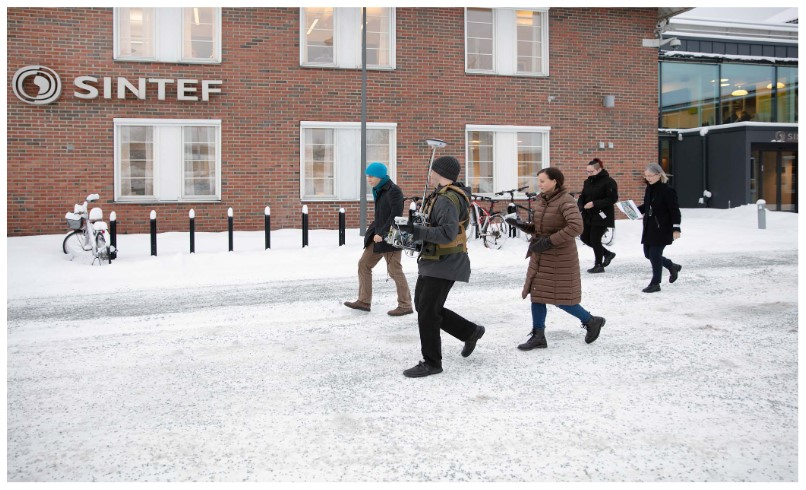
\includegraphics{fig10.jpg}
    \caption{Collaborative navigation team and equipment in a test
campaign.}
    
\end{figure}   
\begin{figure}
    \centering
    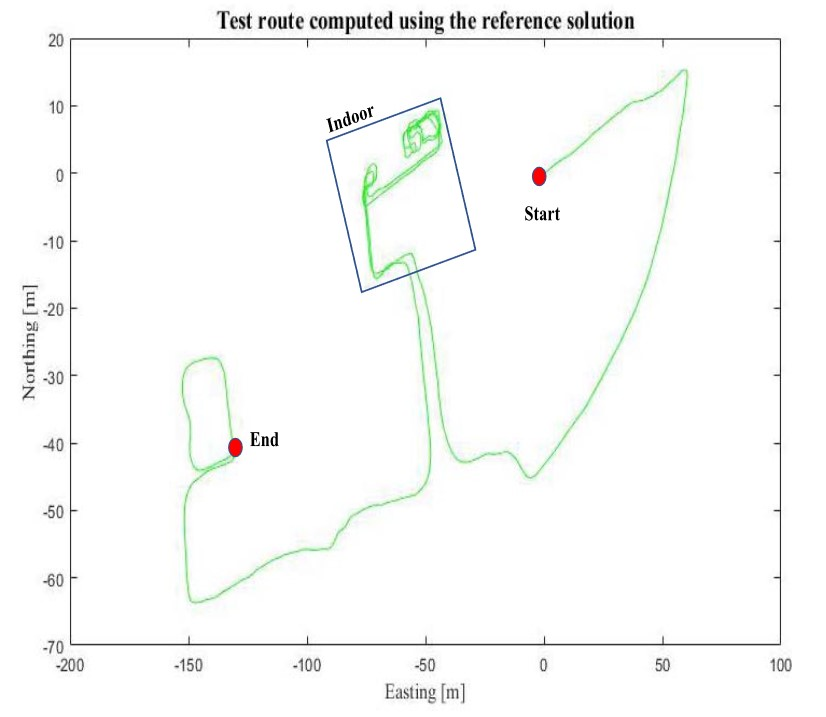
\includegraphics{fig11.jpg}
    \caption{Test campaign route computed using the reference solution.
Start and end positions are shown with red dots and the indoor area with
a blue square.}
    
\end{figure}  
Testing was carried out using a team of collaborating users each carrying a combined navigation system
based on an ADIS16488A tactical grade Micro-Electro-Mechanical (MEMS) IMU, a uBlox M8T multi-constellation
GNSS receiver (GPS, Glonass, Galileo, Beidou), barometer
(integrated within the ADIS16488A), and two forms of
RTT measurement and communication radios. The first radio
operates on 802.15.4a Chirp Spread Spectrum (CSS) in the
2.4 GHz band, while the Second based on the decawave
DW1000 IC uses a 500 MHz UWB pulse implementation.
The RealSense D435 camera was carried by a single user
designated ‘user 1’ rigidly mounted to a carrying frame which
also carried the reference navigation system as shown in
Figure 4.3.\\
\begin{figure}
    \centering
    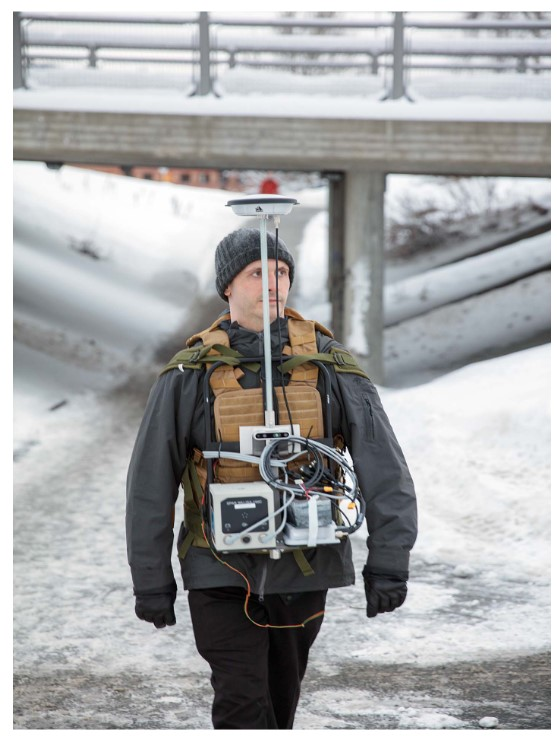
\includegraphics{fig12.jpg}
    \caption{System setup in our collaborative navigation test campaign.}
    
\end{figure} 
The reference system comprised a Novatel SPAN sys-
tem with professional GNSS receiver and ISA100C IMU,
which was initialized outdoors using GNSS Real-time Kine-
matic (RTK) corrections. Figure 4.4 shows a block-diagram
of the system setup and communication between the modules.\\
\begin{figure}
    \centering
    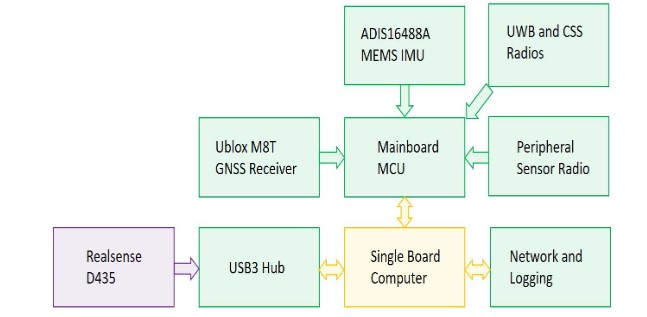
\includegraphics{f9.jpg}
    \caption{Block-diagram of the system setup and communication between
the modules. MCU stands for Microcontroller Unit and CSS Chirp Spread
Spectrum.}
    
\end{figure} 
Solution
was post-processed to form a reference trajectory accurate
and consistent to the decimeter level through the course of
the trajectory including the more than five minutes of GNSS
signal absence when operating within the building. Using this
trajectory it is possible to calculate the navigation state errors
of the collaborative navigation system, as well as the fixed
Realsense camera solution. While the reference system only
directly measures the navigation errors of the primary user
directly, the test trajectory was configured such that secondary
users would follow the same trajectory until stopping at
staggered locations while the primary user proceeded with the
remaining group. At the end of the indoor trajectory segment,
the primary user exited on to the roof, for 30 seconds before doubling back and retracing the trajectory in reverse. This
approach allows approximation of the errors of the secondary
users even absent direct measurement though with increased
uncertainty. For the remainder of the paper we will focus on
the error distribution of the primary user with the camera.

\section{Results}    
First, they computed the visual odometry stand-alone solution. From 6740 images, the solution was
evaluated to be error free for 4269 images. Pedestrians were
detected from 2448 images using the YOLOv2 detector. Kaze
features were successfully detected from 350 images when
detection of SURF points failed, but no features were detected
from 192 images.To evaluate the accuracy of this visual odometry solution,
authors computed user’s speed from the translation from visual
odometry and respective image rate. Speed was compared
with the reference speed solution. \\
The visual odometry speed profile follows the ground truth
speed profile quite well except for two sections, roughly for
images 300-350 and 3800-3850. The reason for the failure
for those parts was the snowy outdoor environment. The
only features closer than 10 meters from the camera, and
thereby usable for the depth computation, were found from
one side of the camera only. This resulted in a degenerated feature configuration and erroneous visual odometry
solution. The speed mean errors were 0.41 m/s for
conventional visual odometry and 0.29 m/s for this solution
and standard deviations 0.60 m/s and 0.43 m/s, respectively.
Thereby, the improvement of the visual odometry solution was
significant in this dataset.\\
To compare this VO solution with the state-of-the-art methods authors have computed an Relative Pose Error (RPE) translation measure that is mainly used for benchmarking VO and
SLAM research. RPE first aligns the two trajectories and then
evaluates directly the absolute pose differences. As their
paper concentrated on solving the challenges arising from the
challenging indoor navigation situations, they computed RPE
for the 288 meters long route indoors. When the VO solution
was lost for longer time for the reasons discussed earlier
they re-initialized the heading using the SPAN system.\\
\begin{figure}
    \centering
    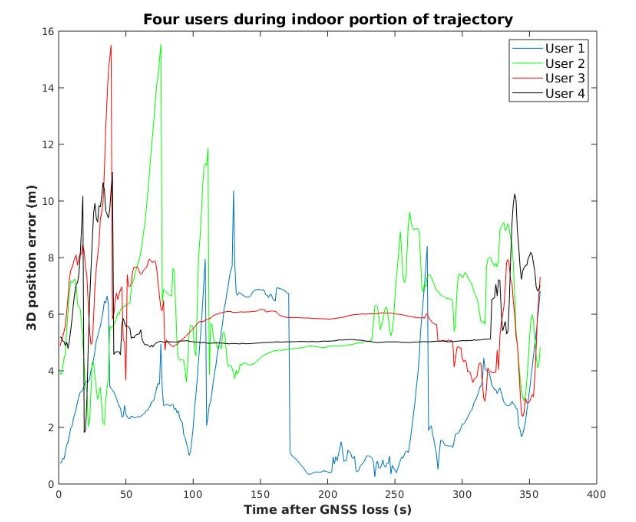
\includegraphics{fig15.jpg}
    \caption{Positioning errors for all users in our cooperative navigation
setup. User number 1 is the user whose position solution is corrected
with the cooperative solution..}
\end{figure}
The
average RPE was 8.8 m and 8.6 m at the end point, resulting
in 3\% error. They computed also the Distance Root Mean
Square (DSRM) measure used in the navigation domain, and
it was 4 m.This VO solution performs provides good performance
when compared to conventional VO solutions using RGB-D
cameras. Using KITTI dataset achieved 5.8\% average
translation error. When the environment is more challenging
for VO and the motion of the camera unconstrained as in
this case, the RPE value increases. In such cases, the error percentages varied between 7\% and even 400\% for short paths
depending on the motion and the environment.Secondly, we computed a loosely coupled visual and inertial
measurement fusion based cooperative navigation solution
using the Extended Kalman filter and
compared that to the reference trajectory.\\
Figure 4.5 shows the positioning error for all users in the cooperative setup,
User1 being the main user computing the visual odometry
solution and getting corrections from the cooperative solution.
On further analysis of the error states of the collaborating
users, it is found that the dominant position errors accumulate
during the portion of the trajectory related to initial building
entry and mirrored in the final building exit. The two factors
that make this section of the trajectory particularly challenging
are that it is simultaneously the longest portion of the trajectory
without the opportunity for the user carried navigation systems
to enter a ZUPT state, but also occurs when the users are
operating in close proximity in a confined and feature poor
stairwell. The consequence of this long ZUPT free trajectory
with a near total lack of useful visual odometry information
providing the large majority of solution error is that the
combined solution is only slightly improved relative to the baseline without the additional visual information in terms of
position error.\\
The root-mean-square (RMS) and maximum errors for the
cooperative solution with (VO) and without visual odometry
(No VO) for all four users are shown in Table 4.1 for the whole
navigation path. What’s important to note with these data
sets is that only user 1 has VO, yet all four of the closely
cooperating users see improvements in their peak, and RMS
error distributions when the VO is activated on only user 1.This shows the ability of one user’s augmentation information
to propagate through the network in an a direct way.
\begin{table}[]
    \centering
       \caption{RMSE And Maximum Errors For All Users In The Cooperative
Navigation Setting With (Vo) And Without (No Vo)
 Visual Odometry.
}
\vline
    \begin{tabular}{c|c|c}
    \hline
         .& VO & No.VO \\
         \hline
        RMS1 & 7.2 & 7.4\\
        RMS2 & 8.1 & 8.2\\
        RMS3 & 8.5 & 8.8\\
        RMS4 & 9.3 & 10.0\\
        \hline
        Max1 & 13.4 & 13.5\\
        Max2 & 13.6 & 13.8\\
        Max3 & 14.2 & 14.6\\
        Max4 & 14.3 & 14.3\\
        \hline
    \end{tabular}
\vline 
    
\end{table}
\chapter{Conclusion}
\setcounter{equation}{1}   

This paper discussed the development of an improved visual
odometry solution, where a small and low-cost RGB-D camera
was used for solving the scale issue, a problem arising when
using a monocular camera. Because the low-cost camera
had inconsistencies in the depth detection, a methods for
making the detection more robust were used. The goal of
the research was to obtain an accurate infrastructure-free
navigation solution for a group of people interacting indoors,
therefore our method detected pedestrians from the images for
avoiding to track their feature points. Accuracy of the resulting
visual odometry solution was significantly improved over the
conventional visual odometry solution for the real-world collaborative navigation dataset. However, the main issue in the
indoor visual odometry, the lack of useful features, remained
at harmful level despite this solution. This led to loosing
the visual odometry solution completely at some challenging
areas, mostly at staircases where the camera was able to
perceive only featureless white wall. Therefore, the fusion of
the visual odometry into the collaborative navigation setup
improved the positioning accuracy only incrementally.\\
Collaborative navigation remains a powerful tool for teams
when entering environments which are unknown and cannot
be prepared for navigation in advance. Therefore, the future
research includes development of deep learning methods for
improving the feature detection in the challenging and feature
poor indoor environment. Then, after solving the remaining
vision based issues authors will continue in fusing tightly the
camera and inertial sensors for the collaborative setting. The
tight fusion of the camera and inertial sensors means that the
feature detection and motion computation phase incorporate
information from the inertial measurement processing and vice
versa, resulting in improved complementary error detection
and mitigation.
